\documentclass[letterpaper,english]{scrreprt}
\usepackage[T1]{fontenc}
\usepackage{graphicx}
\usepackage{float}

\begin{document}
\begin{figure}[H]
	\centering
	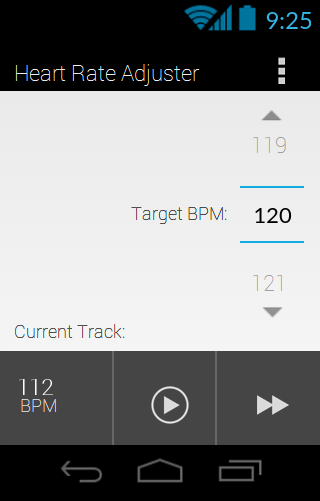
\includegraphics{mobile_ui/1.png}
	\caption{The main screen of the app provides a menu button, a selector for Target BPM, a display of the current track, a display of the current BPM, and the option to Play/Pause and Skip the current track.}
\end{figure}

\begin{figure}[H]
	\centering
	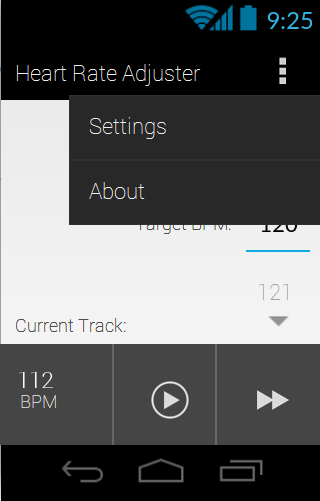
\includegraphics{mobile_ui/2.png}\\
	\caption{Pressing the menu button opens the context menu, providing the option to edit settings and view information about the app.}
\end{figure}

\begin{figure}[H]
	\centering
	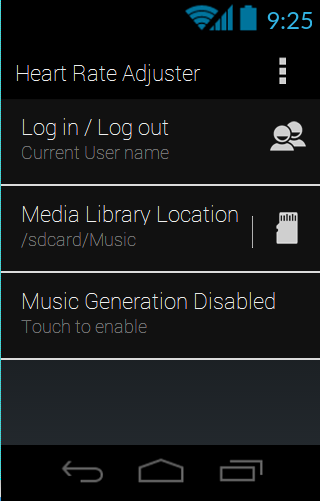
\includegraphics{mobile_ui/3.png}\\
	\caption{The settings page allows the user to open a menu to Log in, to edit the location of the media library (this is done via the OS's directory selection), and configure additional parameters such as music generation (if there is time to implement this feature).}
\end{figure}

\begin{figure}[H]
	\centering
	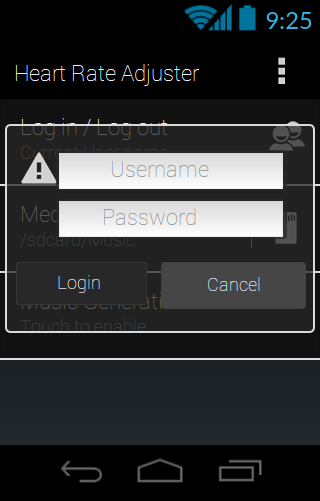
\includegraphics{mobile_ui/4.png}\\
	\caption{Selecting the Log in option prompts the user for their credentials.}
\end{figure}

\begin{figure}[H]
	\centering
	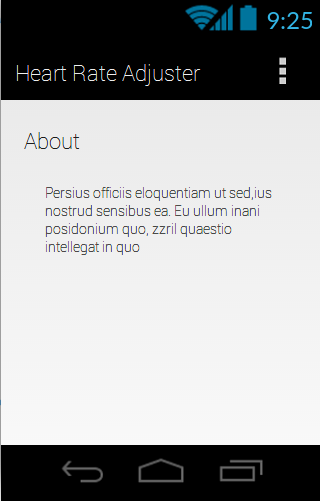
\includegraphics{mobile_ui/5.png}\\
	\caption{Selecting the About option from the context menu provides a description of the application.}
\end{figure}

\end{document}
